\begin{figure}[H]
	\centering
	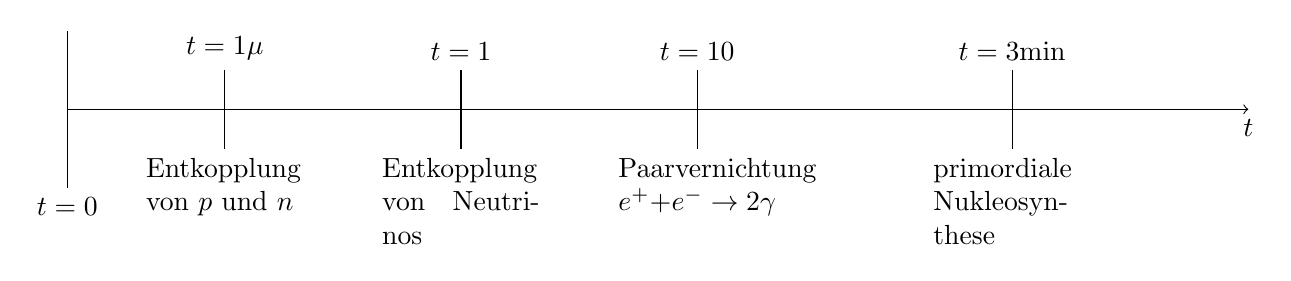
\begin{tikzpicture}
		\draw[->] (0,-1)node[below]{$t=\SI{0}{\s}$}--++(0,2)++(0,-1)--++(2,0)++(0,-0.5)node[below]{\begin{minipage}{2cm} Entkopplung von $p$ und $n$\end{minipage}}--++(0,1)node[above]{$t=\SI{1}{\mu\s}$}++(0,-0.5)--++(3,0)++(0,-0.5)node[below]{\begin{minipage}{2cm} Entkopplung von Neutrinos\end{minipage}}--++(0,1)node[above]{$t=\SI{1}{\s}$}++(0,-0.5)--++(3,0)++(0,-0.5)node[below]{\begin{minipage}{2cm} Paarvernichtung $e^++e^-\to 2\gamma$\end{minipage}}--++(0,1)node[above]{$t=\SI{10}{\s}$}++(0,-0.5)--++(4,0)++(0,-0.5)node[below]{\begin{minipage}{2cm} primordiale Nukleosynthese\end{minipage}}--++(0,1)node[above]{$t=\SI{3}{\min}$}++(0,-0.5)--++(3,0)node[below]{$t$};
	\end{tikzpicture}
\end{figure}
\begin{enumerate}[label={$(\arabic*)$}]
	\item Deuteriumbildung $\text{D}=\text{\textsuperscript{2}H}$
		\begin{equation*}
			p+n\to D+\gamma \text{ mit Bindungsenergie $E_b=\SI{2.225}{M\eV}$}
		\end{equation*}
		\begin{itemize}
			\item Aber: Erst wenn $k_BT\approx E_b$ kann Deuterium in größeren Mengen vorhanden sein, da bei höheren Temperaturen Photodissoziation dominiert
			\item Dies geschieht bei $T\sim \SI{8e8}{\K}$ bzw. $t=\SI{3}{\min}$
			\item Zu diesem Zeitpunkt beträgt das Verhältnis $\frac{n_n}{n_p}\approx\frac{1}{7}$, danach werden praktisch alle Neutronen in $D$ gebunden
		\end{itemize}
	\item Helium-Häufigkeit:
		\begin{align*}
			&\begin{aligned}&\left\{\begin{aligned}\text{D}+\text{D}&\to\text{\textsuperscript{3}He}+n\\
			\text{\textsuperscript{3}He}+\text{D}&\to\text{\textsuperscript{4}He}+p\end{aligned}\right.\\
			&\left\{\begin{aligned}\text{D}+\text{D}&\to\text{\textsuperscript{3}H}+p\\
			\text{\textsuperscript{3}H}+\text{D}&\to\text{\textsuperscript{4}He}+n\end{aligned}\right.\end{aligned} & &\begin{aligned}\text{insgesamt } 3D&\to\text{\textsuperscript{4}He}+p+n \\ E_b&\approx\SI{28}{M\eV}\end{aligned}
		\end{align*}
		Praktisch alle vorhandenen Neutronen werden so in \textsuperscript{4}He gebunden. ($t=\SI{3}{\min}$)
		\begin{itemize}
			\item Anzahldichte von \textsuperscript{4}He:
				\begin{align*}
					n_\text{He}&=\frac{1}{2}n_n \text{ (da e Neutronen in jedem \textsuperscript{4}He)}\\
					n_\text{H}&=n_e-n \text{Anzahldichte von Protonen nach Bildung von \textsuperscript{4}He}
				\end{align*}
				\begin{itemize}
					\item Massenanteil von \textsuperscript{4}He an der Baryonendichte:
						\begin{equation*}
							y=\frac{4n_\text{He}}{4n_\text{He}+n_\text{H}}=\frac{2n_n}{n_p+n_n}=\frac{2\cdot\frac{n_n}{n_p}}{1+\left(\frac{n_n}{n_p}\right)}\approx\num{0.25}
						\end{equation*}
						Etwa $\frac{1}{4}$ der baryonischen Materie im Universum sollte als \textsuperscript{4}He gebunden sein! Dies ist eine robuste Vorhersage der Big-Bang-Modelle und in Übereinstimmung mit Beobachtung VI, Abschnitt (4.1)!
				\end{itemize}
		\end{itemize}
	\item Der Baryonenanteil im Universum
		\begin{figure}[H]
			\centering
			\begin{tikzpicture}
				\node[name=p,draw,rectangle] at (0,0){$p$};
				\node[name=d,draw,rectangle] at (2,0){D};
				\node[name=H3,draw,rectangle] at (4,0){\textsuperscript{3}H};
				\node[name=n,draw,rectangle] at (2,-2){$n$};
				\node[name=he3,draw,rectangle] at (2,2){\textsuperscript{3}He};
				\node[name=he4,draw,rectangle] at (2,4){\textsuperscript{4}He};
				\node[name=li5,draw,rectangle] at (6,6){\textsuperscript{7}Li};
			\end{tikzpicture}
		\end{figure}
		\begin{itemize}
			\item \textsuperscript{5}Li, \textsuperscript{8}Be keine stabilen Kerne
				\begin{align*}
					&\Rightarrow \text{\textsuperscript{4}He}+\text{\textsuperscript{4}He}\to\text{ instabil}\\
					&\Rightarrow \text{\textsuperscript{4}He}+p\to\text{ instabil}
				\end{align*}
				\begin{itemize}
					\item Nach 4 Minuten: $\SI{25}{\%}$ \textsuperscript{4}He, $\SI{75}{\%}$ $p$ und Spuren von D, \textsuperscript{3}He, \textsuperscript{7}Li
				\end{itemize}
			\item Dichte von \textsuperscript{4}He und D hängt von $\Omega_b$ ab:
				\begin{itemize}[label={\textbullet}]
					\item je größer $\Omega_b$, desto größer $\eta$, desto früher kann sich D bilden, desto größer $\frac{n_n}{n_p}$ und $Y$
					\item je größer $\Omega_b$, desto größer ist $n_b$ und desto effektiver die Umwandlung von D in \textsuperscript{4}He $\Rightarrow$ weniger D
				\end{itemize}
				\begin{figure}[H]
					\centering
					\begin{tikzpicture}
						\draw[->] (0,0)--++(2,0)++(0,-0.5)--++(0,1)node[above]{$\num{0.005}$}++(0,-0.5)--++(3,0)++(0,-0.5)--++(0,1)node[above]{$\num{0.01}$}++(0,-0.5)--++(2,0)++(0,-0.5)--++(0,1)node[above]{$\num{0.02}$}++(0,-0.5)--++(2,0)++(0,-0.5)--++(0,1)node[above]{$\num{0.03}$}++(0,-0.5)--++(1,0)node[below right]{$\Omega_bh^2$};
						\draw (0,0)--++(0,-0.5)++(-0.5,0)node[left]{$\num{0.21}$}--++(1,0)++(-0.5,0)--++(0,-1)++(-1,0)node{$Y$}++(1,0)--++(0,-1)++(-0.5,0)node[left]{$\num{0.22}$}--++(1,0)++(-0.5,0)--++(0,-0.5)++(0,-1)--++(0,-0.5)++(-0.5,0)node[left]{$10^{-4}$}--++(1,0)++(-0.5,0)--++(0,-1)++(-1,0)node{$\frac{n}{n_\text{H}}$}++(1,0)--++(0,-1)++(-0.5,0)node[left]{$10^{-5}$}--++(1,0)++(-0.5,0)--++(0,-0.5)++(0,-1)--++(0,-0.5)++(-0.5,0)node[left]{$10^{-9}$}--++(1,0)++(-0.5,0)--++(0,-2)++(-0.5,0)node[left]{$10^{-10}$}--++(1,0)++(-0.5,0)--++(0,-0.5);
						\draw[densely dashed] (6.5,0)--(6.5,-11)(9,-11)--(9,0);
						\fill[pattern=north east lines] (6.55,0)rectangle(8.95,-11);
						\draw[thick] (4,-0.75)rectangle(9.5,-2.25);
						\draw[domain=0:9.5,samples=50] plot({\x},{-3*exp(ln(0.75/3)/9.5*\x)})(3,-1.5)node{\textsuperscript{4}He};
						\draw[thick] (6.5,-5.75)rectangle(9,-7);
						\draw (2,-4)--(9,-7)node[midway,above right]{D};
						\draw[thick] (1.5,-8)rectangle(10,-10.5);
						\fill[draw=black,pattern=north west lines] (1,-8.75) parabola bend (3,-9.75) (10,-8) -- (10,-8.5) parabola bend (3,-10.25) (1,-9.25) -- cycle;
						\node[above left] at (3,-9.75){\textsuperscript{7}Li};
					\end{tikzpicture}
				\end{figure}
			\item bemerkenswerte Übereinstimmung zwischen Theorie und Messungen für die drei Kerne
			\item bisher beste Messung für D:
				\begin{equation*}
					\num{0.012}\leq\Omega_bh^2\leq\num{0.019}
				\end{equation*}
				\begin{itemize}
					\item $\Omega_b\approx\num{0.03}-\num{0.04}$
				\end{itemize}
			\item Aber $\Omega_m>\num{0.1}\Rightarrow$ größter Teil der Materie ist nicht-baryonische dunkle Materie!
			\item Neutrinos ein Kandidat für dunkle Materie?\\
				$\to$ siehe Übung
			\item bester Kandidat als Knstituent für dunkle Materie: WIMPs (=weakly interacting massive particles)
			\item experimenteller Nachweis steht (noch?) aus
		\end{itemize}
\end{enumerate}
\subsubsection{Rekombination}
\begin{itemize}
	\item Nach ca. $\SI{3}{\min}$ ist die primordiale Nukleosynthese abgeschlossen $T\sim\SI{8e8}{\K}$
	\item Bei $z\approx z_{eq}\approx\SI{23900}{\Omega_mh^2}$ beginnt die Materie (d.h. der Staub) zu dominieren. Dhaer wird (F1) zu:
		\begin{equation*}
			H^2(t)\approx H_0^2\frac{\Omega_m}{a^3}
		\end{equation*}
	\item Ansatz $a(t)\sim t^\beta$ ergibt $\beta=\frac{2}{3}$ und damit:
		\begin{equation*}
			a(t)=\left(\frac{3}{2}\sqrt{\Omega_m}\cdot H_0\cdot t\right)^\frac{2}{3}
		\end{equation*}
		für $a_{eq}<<a<<1$
	\item nächste wichtige Schwelle: $T\sim\SI{3000}{\K} (\hat{=} t\sim\SI{3e5}{a})$\\
		Rekombination $p+e^-\to$ neutraler Wasserstoff
	\item Aber: Rekombination Konkurriert mit der Ionisation neutraler Atome durch energetische Photonen
	\item Rekombination findet über einen Zwei-Photonen-Zerfall statt $\Rightarrow$ diese Photonen sind nicht energetisch genug, um ein Atom vom Grundzustand anzuregen
	\item Reaktionsrate des $2\gamma$-Zerfalls $=10^{-8}$. Reaktionsrate des direkten Ly$\alpha$-Übergangs
		\begin{itemize}
			\item Rekombination findet erst spät statt (bei $T\approx\SI{3000}{\K}$)\\
				$(E_\text{ion}(\text{H})=\SI{13.6}{\eV}\hat{=}T=\SI{1.6e5}{\K})$
		\end{itemize}
	\item Ionisationsgrad:
		\begin{align*}
			x&=\frac{\text{Anzahldichte der freien } e^-}{\text{Anzahldichte der insgesamt vorhandenen Protonen}}\\
			&=\num{2.4e-3}\cdot\sqrt{\frac{\Omega_mh^2}{\Omega_bh^2}}\cdot\left(\frac{z}{1000}\right)^{\num{12.75}}
		\end{align*}
		zwischen $\num{800}\leq z \leq \num{1200}$\\
		$x$ ändert sich sehr schnell in Abhängigkeit von $z$ (von $x=1$ zu $x\sim 10^{-4}$)
	\item $x\sim 10^{-4}$ bleibt übrig aufgrund der Expansion (Dichte des Universums wird zu klein)
	\item Das Universum wird \textbf{transparent} für Photonen der Energie
		\begin{equation*}
			E_\gamma\leq\SI{13.6}{\eV}\quad(\text{bzw. }\lambda\geq\SI{121.6}{n\m})
		\end{equation*}
	\item optische Tiefe für die Thomson-Streuung
		\begin{equation*}
			\tau(z)=\num{0.37}\cdot\left(\frac{z}{1000}\right)^{\num{14.25}}
		\end{equation*}
		\begin{itemize}
			\item Photonen mit $z\leq 1000$ breiten sich bis heute aus ohne wesentlich mit Materie zu wechselwirken (Dicke des Übergangs $\Delta z\approx\num{60}$)
			\item Mit Hilfe von Photonen können wir das Universum nur bis $z\lesssim 1000$
			\item Kosmsicher Mikrowellenhintergrund, der isotrop ist (siehe Beobachtung VI und VII, Abschnitt 4.1)
		\end{itemize}
	\item Zwischen $z\sim 1000$ und $z\sim 6$ muss eine Reionisation des intergalaktischen Mediums stattgefunden haben, sonst würden wir keine UV-Photonen von Quellen mit hohem $z$ erhalten (sonst hätte man Absorption durch Photoionisation von neutralem Wasserstoff)
	\item Reionisation passierte (vermutlich) bei $z\sim 17$ durch eine erste Generation von Sternen
\end{itemize}
